\documentclass[12pt,a4paper]{report}
\usepackage{vntex} % Tiếng Việt
\usepackage{graphicx} % Chèn hình ảnh
\usepackage{fancyhdr} % Gói hỗ trợ tạo header và footer fancy
\usepackage{changepage} % Thay đổi lề

% Chèn code
\usepackage{listings} % Thêm gói listings để chèn code
\usepackage{xcolor} % Màu cho code
\lstset{
    language=Matlab,
    basicstyle=\footnotesize\ttfamily,
    numbers=none,
    numberstyle=\tiny\color{gray},
    stepnumber=1,
    numbersep=0.01pt,
    tabsize=2,
    breaklines=true,
    breakatwhitespace=false,
    xleftmargin=0cm, % for line numbers
    framexleftmargin=0cm, % for code frame
    keywordstyle=\color{blue},
    commentstyle=\color{green},
    stringstyle=\color{orange},
    frame=single,
    rulecolor=\color{black},
    basicstyle=\ttfamily,
}

% Footnote, reference and appendix
\usepackage[style=numeric,backend=biber]{biblatex} % Sử dụng gói biblatex
\usepackage{capt-of} %  Footnote trong caption
\usepackage[perpage]{footmisc} % Đánh số lại chú thích mỗi trang
\usepackage[toc,page]{appendix}

% Thiết lập bảng
\usepackage{array} % Gói hỗ trợ các bảng phức tạp
\usepackage{tabularx}
\usepackage{longtable} % Tạo bảng qua nhiều trang
\usepackage{cellspace}
\usepackage{diagbox} % Gói hỗ trợ tạo các ô chéo trong bảng
\usepackage{multirow}
\usepackage{makecell}
\usepackage{adjustbox}

% Thiết lập công thức toán học
\usepackage{amsmath} % Gói hỗ trợ các công thức toán học
\usepackage{amsfonts} % Gói hỗ trợ các ký hiệu toán học
\usepackage{amssymb} % Gói hỗ trợ các ký hiệu toán học
\usepackage{graphicx} % Gói hỗ trợ chèn hình ảnh
\usepackage{bm} % Chữ in đậm trong công thức toán 
\usepackage{physics}

% Thiết lập khác
\usepackage{tikz}
\usepackage{color}
\usepackage{subcaption}
\usepackage{framed}
\usepackage{float} % Để chèn hình ảnh vào đúng vị trí
\usepackage{fancyvrb} % Đưa dữ liệu dạng nguyên thủy vào

% Thiết lập kích thước
\usepackage{geometry}
\geometry{
    left=3cm,
    right=2cm,
    top=2.5cm,
    bottom=2.5cm,
}
\usepackage{hyperref} %Chèn link
\hypersetup{urlcolor=black,linkcolor=black,citecolor=black,colorlinks=true} % Màu cho các đường nét
\everymath{\color{black}}
\setlength{\headheight}{20pt}
\pagestyle{fancy}

%Header
\fancyhead{} % clear all header fields
\fancyhead[L]{
 \begin{tabular}{rl}
    \begin{picture}(25,15)(0,0)
    \put(0,-8){
\includegraphics[width=12mm, height=12mm]{pictures/hcmut.png}}
    %\put(0,-8){\epsfig{width=10mm,figure=hcmut.eps}}
   \end{picture}&
	%
\includegraphics[width=8mm, height=8mm]{hcmut.png} & %
	\begin{tabular}{l}
		\textbf{\bf \ttfamily Trường Đại Học Bách Khoa - ĐHQG TP.Hồ Chí Minh}\\
		\textbf{\bf \ttfamily Khoa Cơ Khí - Bộ môn Cơ điện tử}
	\end{tabular} 	
 \end{tabular}
}
\fancyhead[R]{
	{\tiny \bf \quad} % Khoảng trắng nhỏ trong header bên phải
}

%Footer
\fancyfoot{} % clear all footer fields
\fancyfoot[L]{\scriptsize \ttfamily Động lực học điều khiển}
\fancyfoot[R]{\scriptsize \ttfamily Trang {\thepage}/9}
\renewcommand{\headrulewidth}{0.3pt}
\renewcommand{\footrulewidth}{0.3pt}
\begin{document}
    \begin{titlepage}   
    \begin{center}
        \vspace*{-2cm} 
        \large
        \textbf{ĐẠI HỌC QUỐC GIA THÀNH PHỐ HỒ CHÍ MINH \\
        TRƯỜNG ĐẠI HỌC BÁCH KHOA\\
        KHOA CƠ KHÍ\\
        BỘ MÔN CƠ ĐIỆN TỬ}\\
        
\includegraphics[width=70mm, height=70mm]{pictures/hcmut.png} \\
        \rule{\linewidth}{0.5mm}\\
        \vspace{0.8cm}
        \Large
        \textbf{BÁO CÁO BÀI TẬP LỚN}\\
        \vspace*{0.5cm}
        \Huge
        \textbf{ĐỘNG LỰC HỌC VÀ ĐIỀU KHIỂN}\\
        \vspace{0.5cm}
        \rule{\linewidth}{0.5mm}\\
        \vspace{0.8cm}
        \vspace{1cm}
        \large
        \textbf{GVHD: PGS. TS. VÕ TƯỜNG QUÂN}\\
        \vspace{0.5cm}
        SINH VIÊN THỰC HIỆN:\\[0.3cm]
        \begin{tabular}{|>{\centering\arraybackslash}m{5cm}|>{\centering\arraybackslash}m{7cm}|>{\centering\arraybackslash}m{5cm}|}
            \hline
            \textbf{Họ và tên} & \textbf{MSSV} \\
            \hline
            Đào Trọng Chân & 2210350 \\
            \hline
            Trần Quang Đạo & 2210647 \\
            \hline
            Võ Hữu Dư & 2210604 \\
            \hline
            Dương Quang Duy & 2210497 \\
            \hline
        \end{tabular}
    \end{center}
        
    \vfill
    \large
    \begin{center}
        TP.HCM, \today
    \end{center}
\end{titlepage}

    \tableofcontents
    \cleardoublepage 
    \chapter{Khảo sát tính ổn định của hệ thống}
Ta có hàm truyền đã tìm được ở trên là:
\[
    G(s) = \frac{4.85}{s^2 + 53.51}
\]
Hệ vòng kín với phản hồi là: 
\[
    T(s) = \frac{G(s)}{1+G(s)} 
\]
Phương trình đặc tính:
\begin{align*}
    &1 + G(s) = 0 \\
    &\Leftrightarrow 1 + \frac{4.85}{s^2 + 53.51} = 0 \\
    &\Leftrightarrow s^2 + 58.36 = 0
\end{align*}
$\Leftarrow$ Hệ không ổn định do hệ số của $s^1$ là 0. 
\section{Biểu đồ Bode}
\[
    G(s) = \frac{4.85}{s^2 + 53.51}
\]
Phân tích:
\begin{itemize}
    \item 1 khâu khuếch đại: K = 4.85.
    \item 1 khâu dao động bậc 2.
\end{itemize}
Tần số cộng hưởng: 
\[
    \omega_n = \sqrt{53.51} = 7.315 (rad/s)
\]
Đặc tính tần số:
\[
    G_1(j\omega) = \frac{4.85}{-\omega^2 + 53.51}
\]
\textbf{Biên độ:}
\[
    M(\omega) = \abs{G(j\omega)} = \frac{4.85}{\abs{-\omega^2 + 53.51}}
\]
\[
    \Rightarrow L(\omega) = 20log(M(\omega)) = 20log(4.85) - 20log(\abs{-\omega^2 + 53.51})
\]
\begin{itemize}
    \item Khi $0<\omega<7.315$: biên độ tăng từ -20.85dB đến $+\infty$
    \item Với $\omega > 7.315$: 
\end{itemize}
\begin{align*}
    &20log(4.85) - 20log(\abs{-\omega^2 + 53.51}) \approx 20log(4.85) - 20log(\omega^2) \\
    &= 20log(4.85) - 40log(\omega) \\
    &\Rightarrow \text{Độ dốc giảm: } -40dB/decade \\
    &\Rightarrow \text{Với } \omega > 7.315: \text{ biên độ giảm từ } +\infty \text{ về } -\infty
\end{align*}
\textbf{Pha:}
\[
    \angle G(j\omega) =
    \begin{cases}
        0 \quad ;\quad \omega < 7{,}315 \\
        -180^\circ \quad ;\quad \omega > 7{,}315 \\
        \text{Pha nhảy từ 0 xuống } -180^\circ \text{ tại } \omega = 7.315
    \end{cases}
\]
\begin{figure}[H]
    \centering
    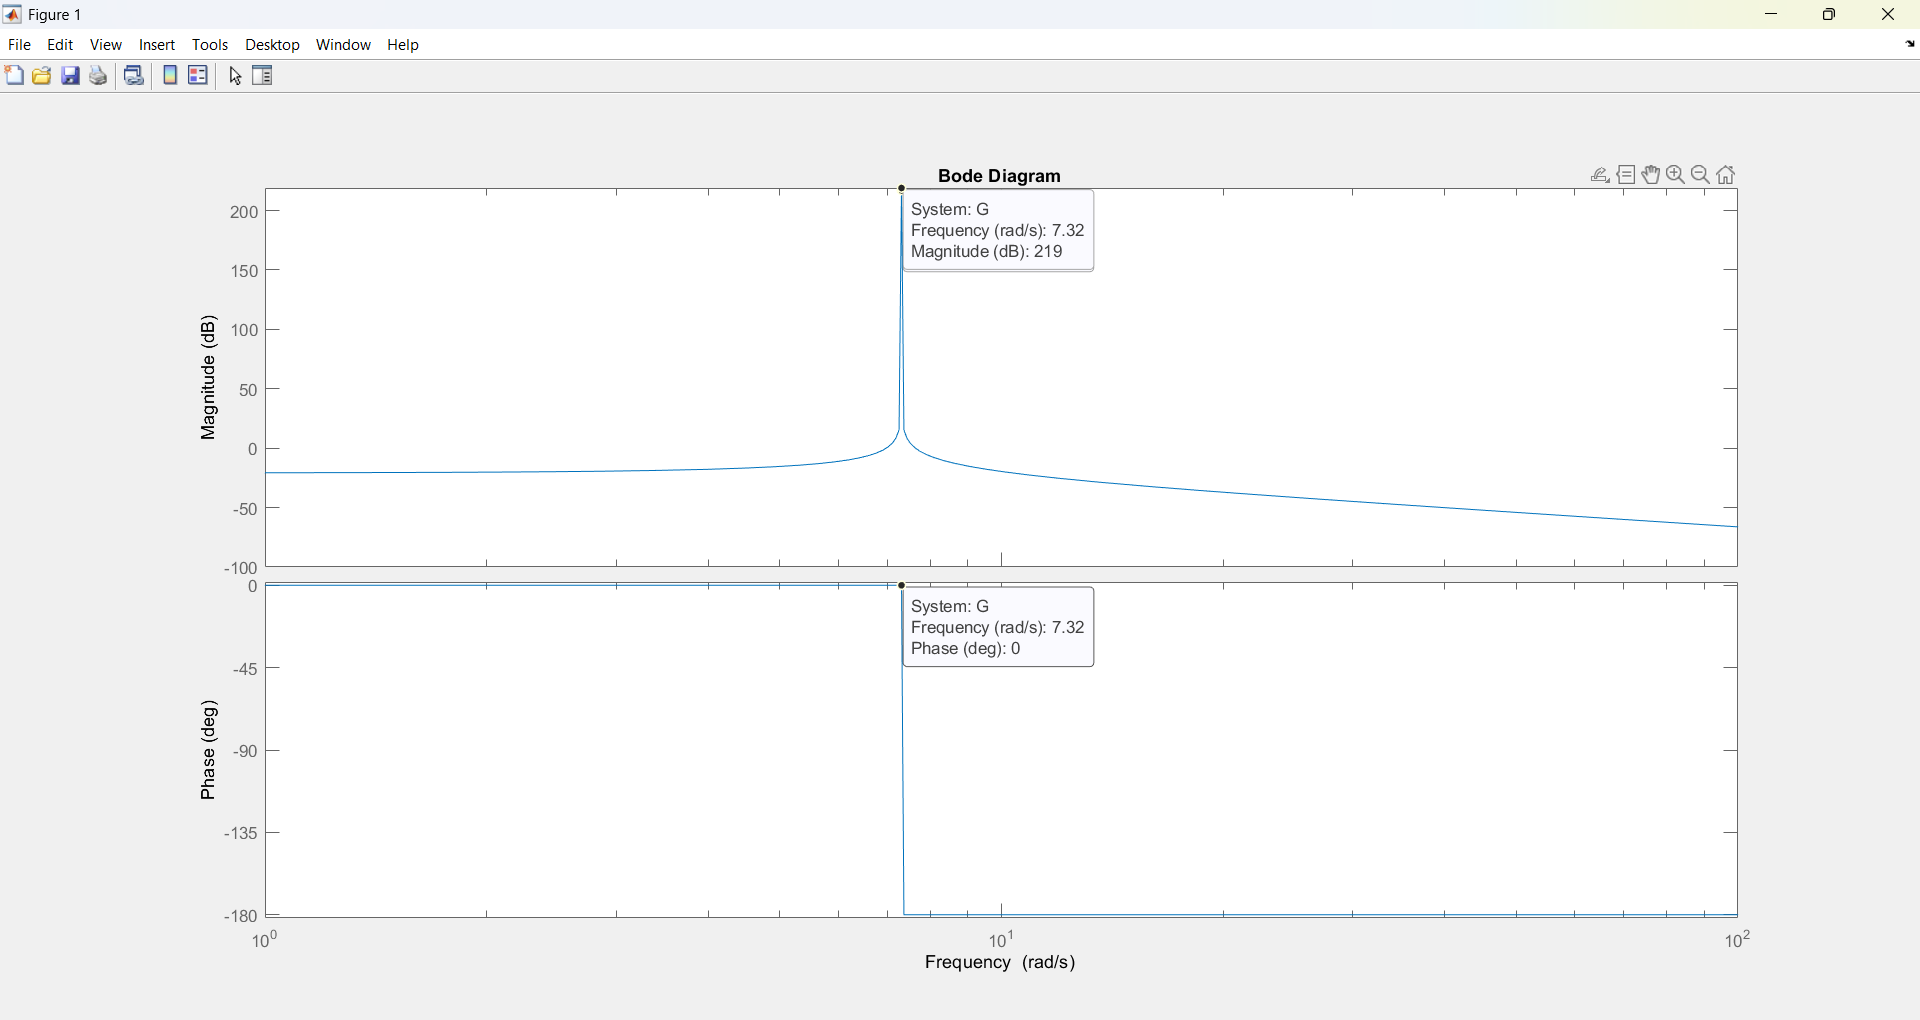
\includegraphics[width=1\textwidth]{pictures/bode.png}
\end{figure}
Nhận xét:
\begin{itemize}
    \item Hệ thống vòng hở: G(s) có các cực trên trục ảo $s=+-7.315$ nên hệ thống ổn định biên. Đồ thị Bode cho thấy biên độ đạt đỉnh tại $\omega=7.315$ và pha nhảy xuống là $-180^\circ$. Điều này xác nhận hệ thống dao động không suy giảm.
    \item Từ độ thị ta có thể thấy độ dữ trữ pha $G_M < 0 dB$ nên đã vi phạm tiêu chuẩn ổn định của biểu đồ Bode $\Rightarrow$ Hệ chưa ổn định. 
\end{itemize}

    \chapter{Đánh giá chất lượng hệ thống điều khiển}
\[
    G(s) = \frac{4.85}{s^2 + 53.51}
\]
\section{Các tiêu chuẩn về xác lập}
Hàm truyền vòng kín:
\[
    T(s) = \frac{G(s)}{1+G(s)} = \frac{4.85}{s^2 + 58.36}
\]
Xét với đầu vào bậc (step input, $R(s)=\frac{1}{s}$), sai số xác lập được tính bằng:
\[
e_{xl} = \lim_{s \to 0} \frac{s \cdot R(s)}{1 + G(s)} 
= \lim_{s \to 0} \frac{1}{1 + k_p} \approx 0{,}92
\]
\begin{center}
    Với $k_p$  là hệ số vị trí, $k_p = \lim_{s \to 0} G(s) \approx 0.09$ 
\end{center}
\end{document}